\documentclass{beamer}
\mode<presentation>
\setbeamertemplate{navigation symbols}{}

% ----------------------------------------------------------------------
%footer
\setbeamertemplate{footline}
{
  \leavevmode
    \hfill
    \usebeamerfont{footer}
    ~~~~~~~~~~~~~~~~~~~~~~~~~~~~~~~~~~
    ~~~~~~~~~~~~~~~~~~~~~~~~~~~~~~~~~~
    \insertframenumber{} / \inserttotalframenumber
    ~~~~~
}

\usepackage[utf8]{inputenc}
\usepackage[T1]{fontenc}
\usepackage[french]{babel}

%figures
\usepackage{graphicx}
\graphicspath{{fig/}}
\DeclareGraphicsExtensions{.eps,.pdf,.jpg}
\usepackage{tikz}

%math
\usepackage{amssymb}
\usepackage{amsmath}

%algo
\usepackage[vlined, linesnumbered, french]{algorithm2e}

% ----------------------------------------------------------------------
%macros

\newcommand{\Z}{{\ensuremath\mathbb{Z}}}
\newcommand{\N}{{\ensuremath\mathbb{N}}}
\newcommand{\R}{{\ensuremath\mathbb{R}}}

\renewcommand{\vec}[1]{\mathbf{#1}}
\newcommand{\ve}[1]{\ensuremath{\vec{e}_{#1}}}

% ----------------------------------------------------------------------
\title[]
 {Optimisation}

\author[T. Roussillon]
 {Tristan Roussillon}

\date{2020}

\institute{INSA Lyon, TC}


%% %rappel du sommaire 
%% \AtBeginSection[]
%% {
%%   \begin{frame}<beamer>
%%     \frametitle{Outline}
%%     \tableofcontents[currentsection]
%%   \end{frame}
%% }

\begin{document}

% ----------------------------------------------------------------------
\begin{frame}
  \titlepage
\end{frame}

% ----------------------------------------------------------------------
\begin{frame}
  \frametitle{Introduction}

  \begin{block}{L'optimisation est partout}
  \begin{itemize}
  \item à la question ``y a-t-il une solution ?'' (pb. de décision)
  \item suit ``quelle est la meilleure solution ?'' (pb. d'optimisation)
  \item l'optimisation peut être sous-jacente : par ex., en apprentissage supervisé, on cherche
    une fonction de prédiction qui minimise une fonction de coût.
    %exemple du salaire d'une personne qui arrive
    %moyenne minimise les écarts quadratiques
    %mediane minimise les écarts absolus
    %mode, cad le plus probable. 
  \item certains problèmes sont difficiles et requièrent des méthodes inhabituelles pour découvrir
    des solutions, mêmes approchées : c'est une partie de ce qu'on appelle l'IA.
  \end{itemize}
  \end{block}
  
\end{frame}

% ----------------------------------------------------------------------
%TODO exemples
% - cf. fiches + ressources tc


% ----------------------------------------------------------------------
\section{\'Enoncé du problème}
% ----------------------------------------------------------------------

\begin{frame}
  \frametitle{Problème d'optimisation}

  \[
  \text{(P)} \left\{
  \begin{array}{c}
    \text{min} \ f(x) \ \text{tel que :} \\
    g_i(x) \leq 0, \ i = 1, \dots, m \\
    x \in S \subseteq \R^n
  \end{array}
  \right.
  \]

  \only<1>{
    \begin{block}{Vocabulaire}
    \begin{itemize}
    \item fonction objectif : $f$
    \item contraintes : $g_i(x) \leq 0, \ i = 1, \dots, m$ et $x \in S$
    \item inconnues : composantes du vecteur $x^T := (x_1, \dots, x_n) \in \R^n$
    \item une solution : $x$ satisfaisant les contraintes
    \item solution optimale/optimum global : une solution minimisant $f$
    \end{itemize}
    %distinction des contraintes en deux:
    %- generalisation a plusieurs classes de pb
    %- traites differement dans les algos
    \end{block}
  }
  \only<2>{
    \begin{block}{Remarques}
    \begin{itemize}
    \item dimension du problème $n \geq 1$
    \item max $f'$ $\Leftrightarrow$ min $-f'$
    \item sans contrainte ($m = 0$) ou avec ($m > 0$)
    \item contraintes d'égalité $g'(x) = 0$ $\Leftrightarrow$ $g'(x) \geq 0$ et $g'(x) \leq 0$
    \item généralement pas d'inégalités strictes
    \end{itemize}
    \end{block}
    %existence de solution (th. de Weierstrass)
    %si f est une fonction reelle continue sur K \subset R^n ferme et borne, alors il existe
    %une solution optimale x \in K qui min f(x)
    %existence aussi si f est une fonction reelle continue et possède la propriété de croissance à l'infini:
    %f(x) -> +inf qs x -> +inf
    %inégalités strictes => ensemble de solutions non ferme et borne, donc possiblement pas de solutions. 
  }
  \only<3->{
    \begin{block}{Résoudre (P) peut être difficile...}
    \begin{itemize}
    \item $n$ peut être grand
    \item l'ensemble des solutions peut être vide, très grand ou infini
    \item $f$ et les $g_i$ peuvent être quelconques %ni differentiable, ni convexe, ni lineaire
    \item $f$ peut être (quasiment) plat autour du min
      %si plat, plusieurs solutions optimales, si quasiment, instabilités numériques 
    \item $f$ peut ne pas être analytiquement connu 
    \end{itemize}
    \end{block}
  }
\end{frame}

\begin{frame}
  \frametitle{Optimum local vs optimum global}

  \begin{block}{Définition}
    La solution $x^0$ est un optimum local du problème (P) s'il existe un voisinage
    $V(x^0)$ autour de $x^0$ tel que $x^0$ soit optimum global du problème
  \[
  \left\{
  \begin{array}{c}
    \text{min} \ f(x) \ \text{tel que :} \\
    g_i(x) \leq 0, \ i = 1, \dots, m \\
    x \in S \alert{\cap V(x^0)}
  \end{array}
  \right.
  \]
  \end{block}

  \begin{exampleblock}{Exemple dans $\R^1$}
    \centering
    \includegraphics[width=0.7\textwidth]{opt-loc}
  \end{exampleblock}
  
\end{frame}


%% % ----------------------------------------------------------------------

%% \begin{frame}
%%   \frametitle{\only<1,2>{Problème d'optimisation}\only<3>{Optimisation continue sans contrainte}\only<4>{Optimisation continue avec contraintes}\only<5>{Optimisation continue convexe}\only<6>{Programmation linéaire}\only<7>{Programmation linéaire en nombre entiers}}

%%   \[
%%   \text{(P)} \left\{
%%   \begin{array}{c}
%%     \text{min} \ f(x) \ \text{tel que :} \\
%%     g_i(x) \leq 0, \ i = 1, \dots, m \\
%%     x \in S \subset \R^n
%%   \end{array}
%%   \right.
%%   \]

%%   \only<1>{
%%     \begin{itemize}
%%     \item fonction objectif : $f$
%%     \item contraintes : $g_i(x) \leq 0, \ i = 1, \dots, m$ et $x \in S$
%%     \item inconnues : $x(x_1, \dots, x_n) \in \R^n$
%%     \item une solution : $\{x\}$ satisfaisant les contraintes
%%     \item solution optimale/optimum global : une solution minimisant $f$
%%     \end{itemize}
%%     %distinction des contraintes en deux:
%%     %- generalisation a plusieurs classes de pb
%%     %- traites differement dans les algos
%%   }
%%   \only<2->{
%%     \begin{itemize}
%%     \item max $f'$ $\Leftrightarrow$ min $-f'$
%%     \item contraintes d'égalité $g'(x) = 0$ $\Leftrightarrow$ $g'(x) \geq 0$ et $g'(x) \geq 0$
%%     \item \only<2,3>{sans contrainte ($m = 0$)} \only<2>{ou} \only<2,4->{avec contrainte ($m > 0$)}
%%     \item diversité de fonctions\only<3->{:} \only<3->{$f$}\only<4->{ et $g_i$} \only<3,4>{continues non linéaires}\only<5>{convexes}\only<6->{linéaires}
%%     \item diversité de $S$\only<3->{:} \only<3-5>{$S \subset \R^n$}\only<3,4>{ continu compact}\only<5>{ convexe}\only<6>{cône de $\R^n$}\only<7>{$S \subset \Z^n$}
%%     \end{itemize}
%%   }
%%   %TODO inégalités strictes ?
%%   %TODO colorer en rouge ce qui apparait
  
%%   %TODO dimension,
%%   %existence de solution (th. de Weierstrass)
%% \end{frame}

%% \begin{frame}
%%   \frametitle{Différentes classes de problèmes et d'algorithmes}

  
%% \end{frame}

% ----------------------------------------------------------------------
\section{Convexité et différentiabilité}
% ----------------------------------------------------------------------
%permet de dire si on peut chercher un min ou un max
%permet de dire si tout optimum local est un optimum global ou non

% ----------------------------------------------------------------------
\begin{frame}<beamer>
  \frametitle{Outline}
  \tableofcontents[currentsection]
\end{frame}


% ----------------------------------------------------------------------
\begin{frame}
  \frametitle{Convexité d'un ensemble}

  \begin{block}{Définition}
    $S \subset \R^n$ est convexe ssi  
    pour tout $x,y \in S$ et $\lambda \in [0,1]$,
    $\lambda x - (1 - \lambda) y \in S$. 
  \end{block}

  \begin{exampleblock}{Exemple pour $S \subset \R^2$}
    \centering
    \includegraphics[width=0.25\textwidth,page=1]{ens-conv} \hspace{0.05\textwidth}
    \includegraphics[width=0.25\textwidth,page=2]{ens-conv}
  \end{exampleblock}
  
\end{frame}

% ----------------------------------------------------------------------
\begin{frame}
  \frametitle{Convexité d'une fonction}

  \begin{block}{Définition}
     Soit $S \subset \R^n$ convexe.
     Une fonction $f : S \rightarrow \R$ est convexe ssi  
    pour tout $x,y \in S$ et $\lambda \in [0,1]$,
    $f(\lambda x - (1 - \lambda) y) \leq \lambda f(x) + (1 - \lambda) f(y)$. 
  \end{block}

  \begin{exampleblock}{Exemple pour $f:\R \rightarrow \R$}
    \centering
    \includegraphics[width=0.45\textwidth,page=1]{fonc-conv} \hspace{0.05\textwidth}
    \includegraphics[width=0.45\textwidth,page=2]{fonc-conv}
  \end{exampleblock}
  
\end{frame}

%% % ----------------------------------------------------------------------
%% \begin{frame}
%%   \frametitle{Programmation convexe}

%%   \begin{block}{Théorème}
%%     Soit $f$ convexe et définie sur $S \subset \R^n$ convexe.
%%     Tout optimum local est un optimum global.  
%%   \end{block}

%%   \begin{exampleblock}{Exemple numérique pour $f:\R \rightarrow \R$}
%%     \only<1>{
%%       $f(x) = x^2 - 6x + 4$\\
%%       $f'(x) = 2x - 6$\\
%%       $f''(x) = 2$ \\ 
%%       ~\\
%%       $\forall x, \ f''(x) > 0 \Rightarrow f$ convexe $\Rightarrow$ $\exists$ un minimum global $x^\star$ tel que:
%%       $f'(x^\star) = 0 \Leftrightarrow x^\star = 3$.
%%     }
%%     \only<2>{
%%       $f(x) = 2x^3 - x^2 + 2x + 5$\\
%%       $f'(x) = 6x^2 - 2x + 2$\\
%%       $f''(x) = 12x - 2$ \\ 
%%       ~\\
%%       On ne peut rien dire de la convexité pour tout $x$.\\
%%       Mais on peut procéder par intervalle. 
%%     }
%%   \end{exampleblock}
  
%% \end{frame}

%% % ----------------------------------------------------------------------
%% \begin{frame}
%%   \frametitle{Différentiabilité en dimension 1}

%%   \begin{itemize}
%%     \item la dérivée seconde est un indicateur de convexité
%%     \item la dérivée première s'annule en un optimum
%%     \item la dérivée première donne même la direction vers laquelle chercher l'optimum
%%   \end{itemize}

%%   \begin{exampleblock}{Exemple numérique pour $f:\R \rightarrow \R$}
%%     \centering
%%     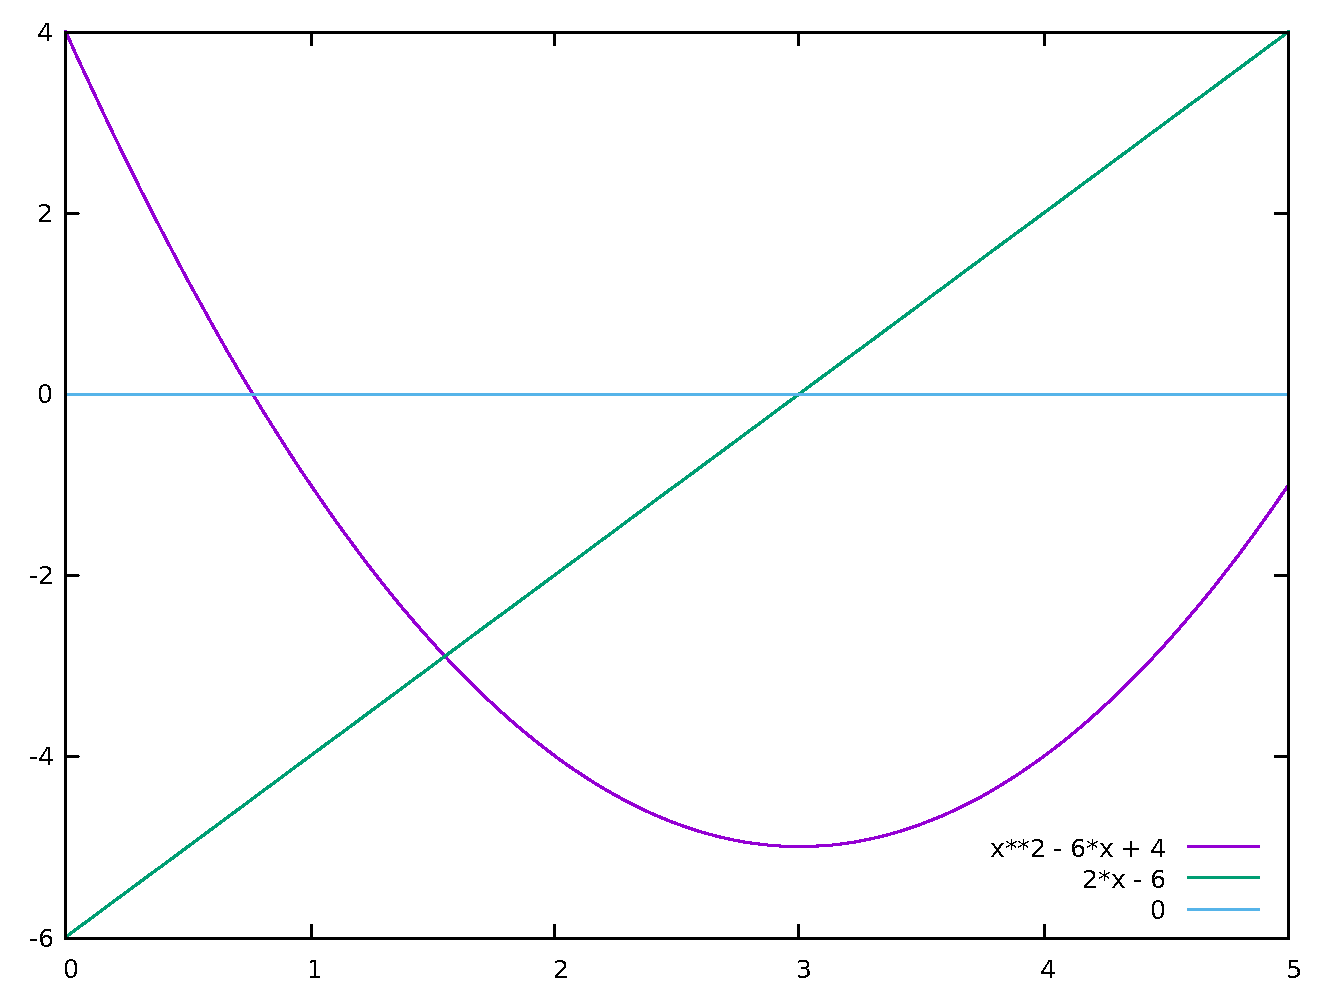
\includegraphics[width=0.6\textwidth]{fonc-plot}    
%%   \end{exampleblock}
  
%% \end{frame}

% ----------------------------------------------------------------------
\begin{frame}
  \frametitle{Différentiabilité pour $f: \R \rightarrow \R$}

  \begin{block}{Dérivée première}
    $f'(x) := \frac{\partial f}{\partial x} = \lim_{h \rightarrow 0} \frac{f(x+h) - f(x)}{h}$.\\
    Géométriquement, c'est la pente de la tangente au graphe de $f$ 
  \end{block}

  {
    \begin{center}
      \includegraphics<+>[width=0.5\textwidth,page=1]{derivee}    
      \includegraphics<+>[width=0.5\textwidth,page=2]{derivee}
    \end{center}
  }
  
  \begin{block}{Dérivée seconde = dérivée de la dérivée première}
    $f''(x) := \frac{\partial f'}{\partial x} = \frac{\partial ^{2}f}{\partial x^{2}}$.
  \end{block}
  
\end{frame}

% ----------------------------------------------------------------------
\begin{frame}
  \frametitle{Différentiabilité pour $f: \R^n \rightarrow \R$}
  
  \begin{block}{Gradient (vecteur), extension de la dérivée première}
    ${\nabla f}^T := (\frac{\partial f}{\partial x_1}, \frac{\partial f}{\partial x_2}, \dots, \frac{\partial f}{\partial x_n})$ \\
    Géométriquement, il est perpendiculaire à la courbe de niveau projetée. 
  \end{block}

  \only<1>{
    \begin{center}
      \includegraphics<+>[width=0.9\textwidth]{gradient}    
    \end{center}
  }
  \only<2>{
    \begin{block}{Hessien (matrice), extension de la dérivée seconde}
      $\nabla^2 f :=
      \begin{bmatrix}{\frac {\partial ^{2}f}{\partial x_{1}^{2}}}&{\frac {\partial ^{2}f}{\partial x_{1}\partial x_{2}}}&\cdots &{\frac {\partial ^{2}f}{\partial x_{1}\partial x_{n}}}\\{\frac {\partial ^{2}f}{\partial x_{2}\partial x_{1}}}&{\frac {\partial ^{2}f}{\partial x_{2}^{2}}}&\cdots &{\frac {\partial ^{2}f}{\partial x_{2}\partial x_{n}}}\\\vdots &\vdots &\ddots &\vdots \\{\frac {\partial ^{2}f}{\partial x_{n}\partial x_{1}}}&{\frac {\partial ^{2}f}{\partial x_{n}\partial x_{2}}}&\cdots &{\frac {\partial ^{2}f}{\partial x_{n}^{2}}}\end{bmatrix}$
    \end{block}
  }
\end{frame}


% ----------------------------------------------------------------------
\begin{frame}
  \frametitle{Différentiabilité et convexité}

  \begin{block}{Théorème}
    Si $f$ est continûment différentiable (deux fois), les conditions 1, 2 (et 3) sont équivalentes:
    \begin{enumerate}
    \item $f$ est convexe,
    \item $\forall x, y, \ f(y) > f(x) + {\nabla f} ^T(x) \cdot (y - x)$,
    \item $\forall x$, le hessien $\nabla^2f(x)$ est une matrice \emph{semi-définie positive},
      c-à-d. ses valeures propres sont \emph{positives ou nulles}.
    \end{enumerate}
  \end{block}

  \begin{block}{Note:}
    Les valeurs propres d'une matrice carrée sont les composantes du vecteur
    $\lambda^T := (\lambda_1, \lambda_2,\dots, \lambda_n)$, solution de
    l'équation $\det{(\nabla^2f(x) - \lambda I)}$.  
  \end{block}

\end{frame}

% ----------------------------------------------------------------------
\begin{frame}
  \frametitle{Conditions d'optimalité générales}

  \begin{block}{Conditions d'optimalité locale}
    Soit $f$ continue et deux fois continûment différentiable en tout $x \in \R^n$.
    $x^\star$ est un optimum local ssi
    \begin{itemize}
    \item ${\nabla f}^T(x^\star) = 0$ (stationnarité) et
    \item $\nabla^2f(x^\star)$ est une matrice \emph{définie positive},
      c-à-d. ses valeures propres sont \emph{strictement positives}.
      %le strictement permet d'éviter les points d'inflexion ou
      %on a un point stationnaire et ou le hessien est seulement semi-definie positive
    \end{itemize}
  \end{block}

  \only<1>{
  \begin{block}{Théorème d'optimalité globale (avec différentiabilité)}
    Soit $f$ convexe et continûment différentiable en tout $x \in \R^n$.
    $x^\star$ est un optimum global ssi ${\nabla f}^T(x^\star) = 0$.
  \end{block}
  }
  \only<2>{
  \begin{block}{Théorème d'optimalité globale (sans différentiabilité)}
    Soit $f$ convexe et définie sur $S \subset \R^n$ convexe.
    Tout optimum local est un optimum global.  
  \end{block}
  }
  
\end{frame}

% ----------------------------------------------------------------------
\begin{frame}
  \frametitle{Exemple numérique pour $f:\R \rightarrow \R$}

    \only<1>{
      $f(x) = x^2 - 6x + 4$\\
      $f'(x) = 2x - 6$\\
      $f''(x) = 2$ \\ 
      ~\\
      $\forall x, \ f''(x) > 0 \Rightarrow f$ convexe $\Rightarrow$ $\exists$ un minimum global $x^\star$ tel que:
      $f'(x^\star) = 0 \Leftrightarrow x^\star = 3$.
    }
    \only<2>{
      $f(x) = 2x^3 - x^2 + 2x + 5$\\
      $f'(x) = 6x^2 - 2x + 2$\\
      $f''(x) = 12x - 2$ \\ 
      ~\\
      On ne peut rien dire de la convexité pour tout $x$.\\
      Mais on peut procéder par intervalle. 
    }
  
\end{frame}

% ----------------------------------------------------------------------
\begin{frame}
  \frametitle{Exemple numérique pour $f:\R^2 \rightarrow \R$}

  \begin{itemize}
  \item $f(x_1,x_2) = x_1^2 + x_2^2 - 4x_1 + 8x_2 - 5$
  \item $\frac{\partial f}{\partial x_1} = 2x_1 - 4, \frac{\partial f}{\partial x_2} = 2x_2 + 8$
  \item $\frac{\partial^2 f}{\partial x_1^2} = 2, \frac{\partial^2 f}{\partial x_1x_2} = 0, \frac{\partial^2 f}{\partial x_2x_1} = 0, \frac{\partial^2 f}{\partial x_2^2} = 2$
  \end{itemize}

  
  $\forall (x_1,x_2), \ \nabla^2f(x_1,x_2) =
  \left(\begin{array}{cc}
    2 & 0 \\
    0 & 2 \\
  \end{array}
  \right)
  $ $\Rightarrow$ $f$ est convexe $\Rightarrow$ \\
  $\exists$ un minimum global $x^\star$ tel que ${\nabla f}^T(x^\star) = 0$, c-à-d.
  \[
  \left\{
  \begin{array}{ll}
    2x^\star_1 - 4 & = 0\\
    2x^\star_2 + 8 & = 0
  \end{array}
  \right.
  \Leftrightarrow x^\star = (2,-4).
  \]
  
\end{frame}


% ----------------------------------------------------------------------
\section{Méthodes numériques d'optimisation sans contrainte}
% ----------------------------------------------------------------------

% ----------------------------------------------------------------------
\begin{frame}<beamer>
  \frametitle{Outline}
  \tableofcontents[currentsection]
\end{frame}

% ----------------------------------------------------------------------
\begin{frame}
  \frametitle{Enoncé du problème}

  \[
  (\text{P}^\circ) \quad
    \text{min} \ f(x), \ x \in \R^n
  \]

  \begin{itemize}
  \item problème fréquent,
  \item même avec contraintes, on peut parfois se ramener à $\text{P}^\circ$,
  \item existence d'une solution optimale si $f$ est continue et :
    \begin{itemize}
    \item soit est définie dans $S \subset \R^n$, fermé et borné,
    \item soit $f(x) \rightarrow \infty$ quand $\|x\| \rightarrow \infty$, 
    \end{itemize}
  \item mais non unicité et nombreux optima locaux pour $f$ quelconque.
  \end{itemize}
  
\end{frame}

% ----------------------------------------------------------------------
\begin{frame}
  \frametitle{Schéma itératif général}

  \begin{itemize}
  \item Soit $f : \R^n \rightarrow \R$ (+ hypothèses)
  \item On part d'une solution initiale $x^{(0)}$
  \item A chaque étape, on obtient une nouvelle solution
    \[ x^{(k+1)} := x^{(k)} - \textcolor{blue}{\lambda^{(k)}} \alert{{\nabla f}(x^{(k)})}, \ \lambda^{(k)} > 0. \]
    (c-à-d. qu'on se déplace dans la direction du \alert{gradient},
    d'un pas d'une certaine \textcolor{blue}{longueur})
  \item On s'arrête quand le gradient s'annule (ou presque)
  \end{itemize}

  ~

  Questions : 
  terminaison ?
  solution initiale ?
  longueur du pas ?
\end{frame}

% ----------------------------------------------------------------------
\begin{frame}
  \frametitle{Longueur du pas}

  \begin{block}{De nombreuses méthodes pour déterminer $\lambda^{(k)}$}
  \begin{itemize}
  \item fixé par l'utilisateur (mais normalisé par la norme du gradient)
  \item $1 / k \|{\nabla f}(x^{(k)})\|$ (le pas diminue au fur et à mesure des itérations)
  \item \emph{Newton}: $\Big( {\nabla^2 f}(x^{(k)}) \Big)^{-1}$
    \begin{itemize}
    \item $x^{(k+1)}$ est l'optimal d'une approximation quadratique en $x^{(k)}$
    \item nécessite le hessien
    \item ne converge pas toujours
    \end{itemize}
  \item \emph{Steepest descent}: tel que $f(x^{(k)} - \lambda^{(k)} {\nabla f}(x^{(k)}))
    = \min_{\lambda \geq 0} f(x^{(k)} - \lambda {\nabla f}(x^{(k)})$
  \end{itemize}
  \end{block}
\end{frame}

%exemples Newton convergence ratée, exemple zigzag

% ----------------------------------------------------------------------
\begin{frame}
  \frametitle{Ce à quoi vous avez échappé}

  \begin{itemize}
  \item Newton modifié et quasi-Newton
  \item méthode du gradient conjugué, méthode de Fletcher et Reeves
  \item méthode de Davidon-Fletcher-Powell (DFP)
  \item méthode de Broyden-Fletcher-Goldfarb-Shanno (BFGS)
  \item algorithme de Powell (sans dérivée)
  \end{itemize}
  
\end{frame}

%TODO
%conditions d'optimalité sans contraintes
% et méthodes de desc. de grad. 
%conditions d'optimalité avec contraintes inegalites: 
% - conditions de Kuhn et Tucker, etc. (p. 204 et après [1])
%conditions d'optimalité avec contraintes egalites: 
% - multiplicateur de Lagrange, etc. (p. 209 et après [1])
% - dualité de Lagrange




% ----------------------------------------------------------------------
\section{Optimisation combinatoire}
% ----------------------------------------------------------------------


\end{document}

